\clearpage\subsection{Horizontal Asymptotes}
Horizontal asymptotes come about because of a range restriction. To be more accurate, horizontal asymptotes are a result of the end behavior of a function as $x$ approaches $\pm \infty$. Just like with vertical asymptotes, we can solve for the range of a function and observe its behavior as it aproaches the range restrictions. Conversely, we can use values from the domain that, when plugged into the function, gradually bring the function closer and closer to its range restriction.

What does this mean? Take the example $g(x) = \dfrac{1}{x}$. Earlier in the section on asymptotes ("1.1 Asymptotes"), we calculated $g(x)$ for extremely large values of $x$. As the value of $x$ increased, the output $g(x)$ decrased. In fact, it slowly got closer and closer to its domain restriction: $y \ne 0$. Let's look at some example problems.

\begin{problem}
    For the function, $f$, defined below, find it's horizontal asymptotes.
    \[
        f(x) = \frac{1}{(x - 1)(x + 3)}
    \]
\end{problem}

\begin{solution}
    The function $f(x)$ cannot equal $0$, regardless of what the denominator is, because the numerator will \textbf{always} be $1$. Therefore, we can say that this method has a range of $y \neq 0$. To see if this is indeed a horizontal asymptote, let's plug some large values and see what happens.
    \[
    \begin{aligned}
        f(100) &\approx 0.0000981
        f(10000) &&\approx 0.000000009998 \\
        f(-100) &\approx 0.000102
        f(-10000) &&\approx 0.00000001
    \end{aligned}
    \]
    We can see that plugging large values of $x$ gets us closer and closer to our range restriction $y \neq 0$. Since that is our only range restriction, we can say that the function $f(x)$ has a horizontal asymptote of $y = 0$.

    \begin{center}
        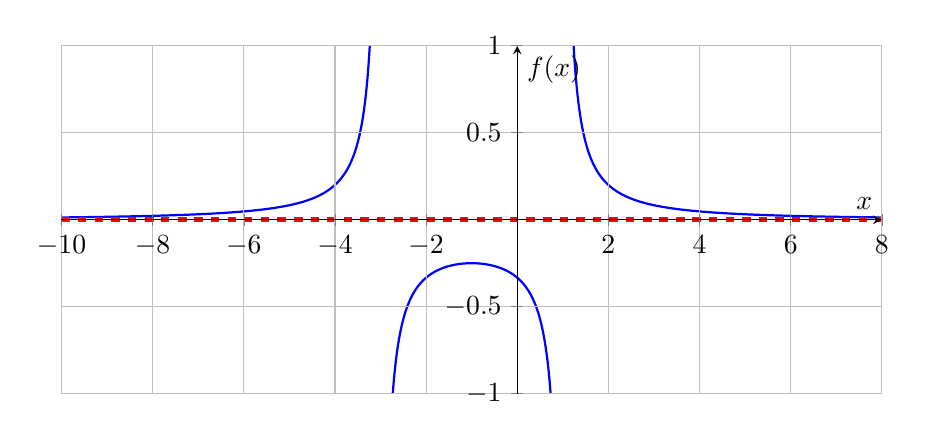
\begin{tikzpicture}
            \begin{axis}[
                axis lines = middle,
                xlabel = $x$, ylabel = {$f(x)$},
                xmin = -10, xmax = 8,
                ymin = -1, ymax = 1,
                grid = both,
                width = 12cm,
                height = 6cm,
                samples = 10,
                smooth,
                axis on top,
            ]
            \addplot[blue, thick, domain=-10:-3.01, samples=300] {1/((x-1)*(x+3))};
            \addplot[blue, thick, domain=-2.99:0.99, samples=300] {1/((x-1)*(x+3))};
            \addplot[blue, thick, domain=1.01:8, samples=300] {1/((x-1)*(x+3))};
            \addplot[red, dashed, ultra thick, domain=-10:8, samples=10] {0};
            \end{axis}
        \end{tikzpicture}
    \end{center}
\end{solution}

\begin{problem}
    For the function, $g$, define below, find it's horizontal asymptotes.
    \[
        g(x) = \frac{3x^2 + 5}{x^2 + 1}
    \]
\end{problem}

Your first instinct would be to look for the range. While that \textit{is} a valid strategy, you'll notice that it's quite cumbersome. I mean... Where do you even start? Throwing a bunch of large values of $x$ \textit{would} give the answer, but let's think of a better way to explain this. It's crucial that we explore this further because it reveals a trick we can use to solve any problem like this in an instant.

\begin{solution}
    First, let's plug the number $1$ into this function.
    \[
        g(1) = \frac{3(1)^2 + 5}{(1)^2 + 1} = \frac{3 + 5}{1 + 1}
    \]
    When we plug $x = 1$ into this function, that $+5$ and $+1$ in the numerator and denominator \textit{really} change the answer. We're jumping from $5$ to $8$ in the numerator and from $1$ to $2$ in the denominator. Now, let's try plugging a larger number, like $100$.
    \[
        g(100) = \frac{3(100)^2 + 5}{(100)^2 + 1} = 
        \frac{3(10000) + 5}{10000 + 1} = \frac{30000 + 5}{10000 + 1}
    \]\clearpage
    Take a look at this. The $+5$ and $+1$ in the numerator and denominator don't really do anything anymore. Yeah, they increase the number, but compared to how large $30000$ and $10000$ are, they're basically nothing. It should be clear, now, that plugging larger and larger numbers into $x$ makes the $+5$ and $+1$ more and more insignificant. As $x$ increases, we're basically looking at
    \[
        g(x) = \frac{3x^2}{x^2} = \boxed{3}
    \]
    Sure enough, that is our asymptote. The horizontal asymptote of $g(x)$ is $y = 3$.

    \begin{center} {\vspace{-0.75cm}}
        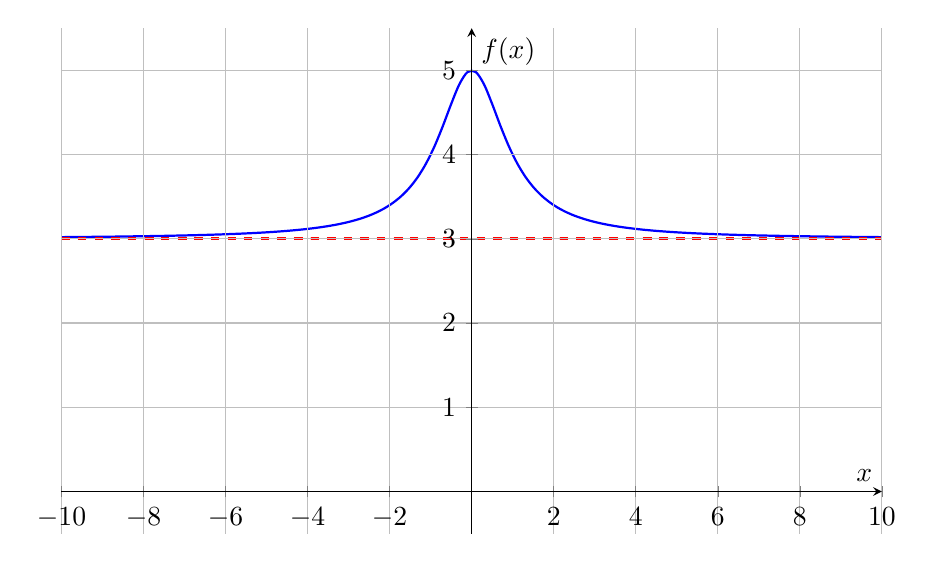
\begin{tikzpicture}
            \begin{axis}[
                axis lines = middle,
                xlabel = $x$, ylabel = {$f(x)$},
                xmin = -10, xmax = 10,
                ymin = -0.5, ymax = 5.5,
                grid = both,
                width = 12cm,
                height = 8cm,
                samples = 50,
                smooth,
                axis on top,
            ]
            \addplot[blue, thick, domain=-10:10, samples=100] {(3 * x^2 + 5) / (x^2 + 1)};
            \addplot[red, dashed, very thick, domain=-10:10, samples=10] {3};
            \end{axis}
        \end{tikzpicture}
    \end{center}
\end{solution}

If the degree of the numerator and denominator are the same, the horizontal asymptote is determined by dividing the coefficient of the highest degree in the numerator by that of the denomianator.